

\documentclass[conference]{IEEEtran}
\ifCLASSINFOpdf

\else
 \fi
 \usepackage{graphicx}
  \usepackage{url} 

\begin{document}
\title{7100 Research Proposal: Machine Listening Module}

\author{
\IEEEauthorblockN{Christopher Latina}
\IEEEauthorblockA{Georgia Tech Center for Music Technology\\
Atlanta, GA\\
Email: chris.latina@gatech.edu}
}

% make the title area
\maketitle

% As a general rule, do not put math, special symbols or citations
% in the abstract
\begin{abstract}
Machine listening provides a set of data with which music can be synthesized, modified, or sonified. Real time audio feature extraction opens up new worlds for interactive music, improvisation, and generative composition. I would like to propose working on a an interdisciplinary project within the realm of composition and engineering. For my master's project, I'm especially interested in the intersection of machine listening with interactive performance using DIY embedded systems, integrating machine listening with analog synthesizers.

\end{abstract}

% no keywords

\IEEEpeerreviewmaketitle



\section{Introduction}

Computer music often deals with some of the fundamental issues found in interface design. Initial iterations are often cumbersome and clumsy. Poor practices can propagate through the production chain and become the de facto. Currently, many state of the art machine listening libraries are embedded into technical albeit high level synthesis languages like Pure Data and SuperCollider. While many competent programmers and musicians can easily build instruments out of them, these techniques live within the screen. In the past few years, there has been a movement towards reclaiming analog technologies, especially voltage controlled synthesis. The Deopfer Eurorack standard has become a more well known phenomenon in the past decade with new eurorack modular startups popping up frequently \cite{idreamof}. The Do It Yourself aesthetic behind this movement has developed from recreating classic circuits of the past to inventing new techniques, especially those with embedded DSP. This platform is popular with musicians and hobbyists because it is hands on: instrument builders and performers want to plug and unplug, turn knobs and watch LEDS blink. This platform is ripe for embedding machine listening techniques within the context of improvisation and composition. 

\section{Motivation}

\begin{figure}
\centering
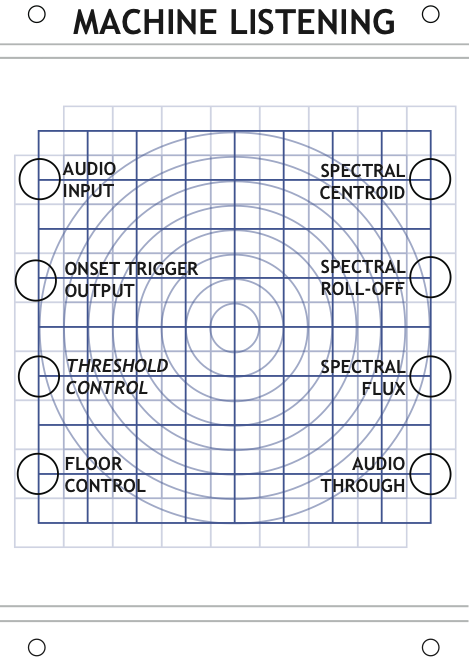
\includegraphics[width=0.4\textwidth]{frontpanel}
\caption{A mockup of the frontpanel for the machine listening module}
\end{figure}

The current state of real time audio feature extraction allows for significant control of synthesis parameters for innovative compositions. The generative works of Mark Fell and Gabor Lazar often employ modernized (computational) versions of west coast synthesis techniques. This method is effective in that the parameters controlling synthesis or effects are aware of the input signal, creating transparent mappings. The text to support his release "Head Office Transformation" on EVOL's ALKU imprint describes an instance of his process.

"I was watching my daughter play on Guitar Hero with headphones, all I could hear was the clicking of the buttons as she played. She, on the other hand, was have a very different experience. I made a recording of the sound of the button pushing which lasted about 30 minutes. Following this I implemented a simple system to analyze the sound file and give me a list of all the timings of the button pushes. This was then used to trigger a simple kick drum sound and lush chord generated using 4 operator FM synthesis. For me the music made outside the headphones, the skeleton of the guitar hero performance was far more interesting that the illusion of skill and performance it offered to the player. A more interesting head space transformation." -- Mark Fell, 'Head Off' \cite{headoff}

With this project, I want to promote the use of machine listening as a compositional tool. Previously, my Signal-Aware Spatial Positioning application gave control to a user to modulate ambisonic sound field rotation using onsets and spectral information from the audio signal itself. I would like to bring this approach into the analog modular world, creating an environment where computational analysis of the audio signal can control synthesis or effects for existing instruments. This will allow musicians to have access to these controls without the overhead of manually routing a microphone or buffer to an audio interface through SuperCollider or Pure Data, mapping control rates from machine listening to OSC / MIDI CC then back out to their VSTs or hardware synths from the DAW. This eliminates the need to rely on multiple programs and facilitates haptic and interactive composition for live performance with these techniques. It also removes the need for a laptop on stage.

Because there has been a resurgence in analog and control voltage-based instruments (see new products from Korg, Elektron, Roland, etc.), this design would enable musicians to easily create analysis-based mappings physically by simply routing the modulation sources (eigth inch +/- 5V cables) to their existing instrument's modulation sources. This allows musicians to focus on performing, rather than making sure their software patch does not crash. Ideally, my module will also send OSC / MIDI CC so that musicians can use this instrument regardless of whether they work with analog or digital instruments.

\section{Related Work}
The idea of building generalized hardware instruments is not a new concept. The MIDI controllers and Max/MSP patches of the early 2000's follow suit. This approach becomes problematic because it is too easy to change: the interface is decoupled from the sound generation and synth itself can be easily modified with it's own set of tools. [TODO REFER TO ROWE re DMIs] Coupling the interface with the synthesis engine is an important design consideration when creating a digital music instrument.

Qu-Bit's Nebulae (early prototypes are referenced in the authors CSounds paper \cite{csounds}) and open-source project Terminal Tedium \cite{terminaltedium} and Mutable Instrument's Clouds modules \cite{mutable} are the first implementations based on the idea of controlling eurorack with affordable open source microcomputers such as the Raspberry Pi, Teensy, and Cortex-M4 ARM processors. A side effect of the Nebulae was the ability to not-so-easily hack the instrument. The instrument's user base is generally technically savvy engineers who figured out how to replace the PureData patches loaded inside with modified firmware to create new sounds. The fact that the instrument is encapsulated but editable creates longevity. Compared with common MIDI instruments, the interface to edit the instrument is not part of the instrument itself.

Lastly, my inspiration comes from a classic west coast synthesis technique, the envelope follower. This technique is common nowadays in side-chained compressors or dynamic processors \cite{Settel1994}. Buchla's 230 Triple Envelope Follower is different in that it generates transient triggers and envelopes from audio signals as a standalone tool, predating real time digital onset detection. I would like to embed real time onset detection along with spectral analysis data into the eurorack format.

\begin{figure}
\centering
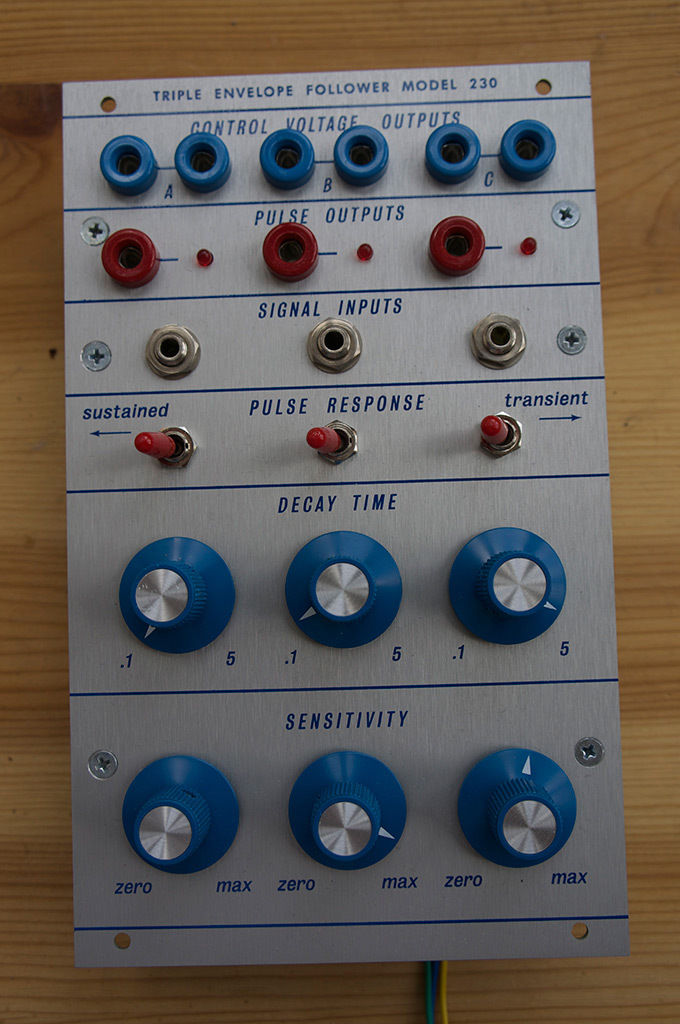
\includegraphics[width=0.4\textwidth]{buchla.jpg}
\caption{Buchla's Model 230 Triple Envelope Follower}
\end{figure}


\section{Context}
For the compositional portion of the project (SuperCollider, analog modular synthesis, video, live performance), my influences include Mark Fell and Gabor Lazar's "The Neurobiology of Moral Decision Making", Lee Fraser's E164 (Entr'acte, 2014), Erik Nystr�m's Morphogenese (empreintes DIGITALes, 2014) and his paper "Textons and the Propagation of Space in Acousmatic Music" \cite{Nystrom2011}. I will elaborate upon this at a later time.

\section{Proposed Method}

I propose a modernized digital version of Buchla's envelope follower using a Raspberry Pi and GPIO. I would like to mimic libraries similar to SuperColliders onsets.kr \cite{nickcollins} and William Brent's bark object \cite{brent2011}, along with realtime spectral/cepstral analysis features such as spectral centroid / rolloff, flatness, and MFCCs \cite{brent2009}. My design will include an audio input and thru signal, a CV trigger output signal, knobs to control threshold and floor, and an output that measures the energy of the signal and spectral data. Following Qu-Bit's and Terminal Tedium's approach to embedded CV-based CSound and Pure Data instruments into the eurorack format, my project will extend the tutorial style format explaining the processes' successes and pitfalls. I will extend my set of tutorials on the github I had created last year.

\begin{figure}
\centering
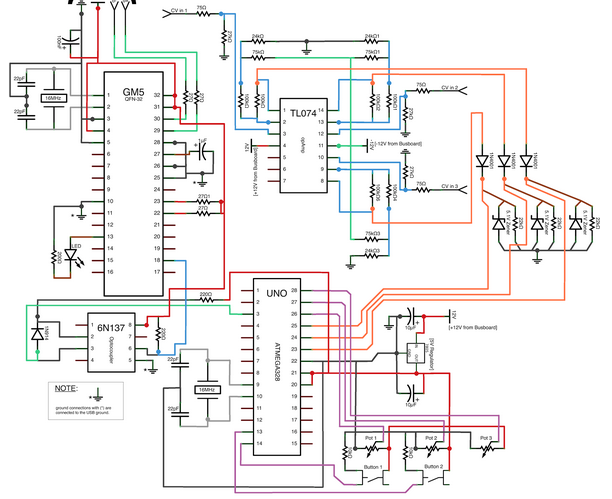
\includegraphics[width=0.45\textwidth]{nebulae.png}
\caption{The guts of the Qu-bit Nebulae \cite{csounds}}
\end{figure}

Below, I've described some use cases for this system

Physical: Capture onsets from piezo sensors. Analyze using C libs in real time, generate eurorack specific control voltages.

Auditory: Take a microphone input to capture energy in the room, technique where the audio may feedback and trigger itself -- the performer can control the master volume and perform the instrument or simply control the synthesis to which control voltages are mapped. Also, can take in pre-composed music or a mic'd instrument and synthesize based on onsets and spectral features. This is the idea of sonifying music. 

As part of the composition, I will research current techniques for interactive music systems along the lines of Robert Rowe's book reflecting upon machine listening and compositional techniques, especially investigating more contemporary ideas of embedding typically laptop-centric techniques into a haptic system, namely a modular system. 

\section{Proposed Evaluation}
Evaluation of latency and evaluation of object as an instrument and an artifact. Evaluation of composition as aesthetically referential and innovative.


\section{Required Resources}
\begin{itemize}
  \item  ArduinoUno+ AVR 28 Pin 20MHz 32K 6A/D - ATMega328P
   \item VoltageRegulator-5V
  \item TI-TL074
  \item 16MHzCOM-00536
  \item caps, resistors, breadboard, pots, eighth inch jacks
  \item PittsburghPowerRails
  \item MeanWellPD-2515
  \item VoltageRegulator-12V
\end{itemize}

\section{Deliverables}
Module, instructions, github repository with code and designs, performance

\section{Timeline}
October
\begin{itemize}
  \item Begin implementation (own framework in C++. Eventually tie in with Pure Data)
  \item Options for debugging / emulations or unit testing
  \item Diagram of program structure / architecture (subject to change)
  \item Begin framework to capture and analyze real time audio input from USB-C
   \item Take a look at Terminal Tedium's GPIO in python to C to Pure Data

\end{itemize}

November
\begin{itemize}
   \item Continue building libraries -- start solidifying prototype. 
   \item Build out Spectral centroid, begin onset implementation
   \item Send messages to PWM library in Python and out of GPIO to 5V Doepfer Standard
   \item Find correct RC filters for correct cutoff
   \item Begin Compositional Piece using Make Noise Function, Optomix + Multifilter
   \item Think about parameterizing features / sample rate. How will this be extensible
   \item Test framework - Evaluation of Libraries
\end{itemize}

January
\begin {itemize}
  \item Finalize design 
  \item Allow features to be changed, edited. Remove Roll-off, replace with timbral features (MFCCs)
  \item Continue building libraries 
\end {itemize}

February
\begin {itemize}
  \item Construct breadboard prototype 
  \item Finalize Libraries
  \item Evaluation of entire device -- latency, etc. (Platform dependent and independent test (on desktop vs. rPi)
  \item Evaluation of it as an instrument, does latency interfere with audio output for mixing / improv /effects.
\end {itemize}

March
\begin {itemize}
  \item Put it together. Finish composition + Paper. Document the composition
\end {itemize}

April 
\begin {itemize}
  \item Rehearse / Perform / Write-up
\end {itemize}

\section{Conclusion}
The idea behind this tool is to create a framework for embedded DIY DSP. The output will be physical and encapsulated to prevent the issue of constant reconfiguration found in software instruments. The evaluation of latency and playability will document places for improvement. This output of this project will be an open-source manual and working prototype of the product. 

\bibliographystyle{acm}
\bibliography{biblio}  % biblio.bib is the name of the Bibliography in this case

*** All linked accessed Monday September 28, 2015
% that's all folks
\end{document}


